\section{Evaluation}
\label{sec:evaluation}

We evaluate \proto by comparing its end-to-end gas cost with other baselines over $35$ popular smart contracts sourced mainly from Etherscan~\cite{etherscan} and OpenZeppelin~\cite{openZeppelin}.
Results show that the code generated automatically by \proto can match the performance of the hand-optimized reference implementation. 
All data are available online ~\cite{data}. The experiments are run on Ganache, a local Ethereum simulator from Truffle~\cite{truffle}.

\subsection{Experimental Setup}

\noindent\textbf{Contract benchmarks.}  
We construct our benchmark by selecting a diverse set of widely used, open-source, and audited contracts from platforms such as Etherscan ~\cite{etherscan} and OpenZeppelin ~\cite{openZeppelin}. The benchmark covers multiple token standards, including ERC20, ERC721, ERC1155, and ERC777, encompassing both simple yet popular contracts and more advanced logic, as well as non-token contracts from domains such as governance, DeFi, utility, and token management.
We aim to ensure that our selection is realistic, widely applicable, and covers a broad range of representative standards and functionalities.
For each benchmark contract, we provide a declarative implementation, with many of them having no prior publicly available declarative counterpart.
We validate and compare our declarative implementations to their original Solidity versions through a unified evaluation suite introduced later.
% We have in total xxx contracts
% We evaluate \proto on 15 open‑source Ethereum contracts that reflect the functional diversity of on‑chain applications. The corpus spans fungible tokens, non‑fungible assets, governance and control primitives, and a compact storage micro‑benchmark.
% For each contract, we rewrote the specification in Datalog, with its public interface identical to that of the corresponding \emph{Reference} Solidity contract, allowing both implementations to be evaluated by the same workload.

% To address some limitations identified in Section~\ref{ssec-limitation}, we extended the DeCon compiler with additional semantics. 
% \proto supports advanced mathematical operators and exposes on‑chain environment variables. Specifically, \emph{SimpleStorage} incorporates several advanced math operations mentioned above with some other contracts incorporating the use of on-chain variables.

\noindent\textbf{Evaluation workload.}
For every contract and each of its transaction types (e.g., \texttt{mint}, \texttt{transfer}), we synthesized a simulation workload based on randomization functions within parameter ranges.  
The evaluation workload for each transaction contains multiple traces, which are executed against a generated pool of Ethereum accounts and include any prerequisite operations (such as initializing account balances) before the tested transaction. Every trace contains multiple valid calls to the targeted transaction, and calculates the mean cost of all the calls (Except the first call, which works as the warm-up and is dropped).
The final gas cost of the transaction is reported as the average gas consumption over all its traces.


\noindent \textbf{Transaction Frequency.} 
For contracts whose transaction frequencies can be extracted from Etherscan~\cite{etherscan} using the most recent 10,000 on‑chain transactions of this contract, we estimate its gas cost as a frequency-weighted average. When these data are unavailable, we instead adopt the unweighted mean over all transaction types. 
This metric is used to evaluate the gas consumption of all \proto's plans and the baseline implementations.

\noindent \textbf{Profiling.} In the experiment, we compare three approaches:
\begin{itemize}
    \item \textbf{\sf Incremental Datalog:} Solidity compiled from vanilla incremental Datalog execution with minimal optimizations.
    \item {\bf \proto:} Solidity compiled from Datalog contracts with the full suite of our optimizations applied.
    \item \textbf{\sf Reference:} Solidity contracts obtained from open‑source repositories. Each has had extensive manual optimizations performed by multiple stakeholders.
\end{itemize}

Note that optimizations of read projection and indexing are not our main focus of research; we also implement them in the {\sf Incremental Datalog}. In addition, since the triggers and records of each transaction are normally not stored by the blockchain, they are not in the domain of materialization and are also excluded from the {\sf Incremental Datalog}.

\noindent \textbf{Profiling overhead.}
Profiling incurs no significant gas costs, and the time overhead is relatively low and manageable. The generation of materialization plans is a one-time process that typically finishes within a minute. With the search space optimized, each contract typically produces a limited number of minimal candidate plans (usually fewer than 10, and found to be at most 16 in our benchmark suite). Generating Solidity code for each plan takes about 1 second, and running simulation workloads for a corresponding transaction requires only a few seconds. In total, all generated variants of a given contract can be profiled within minutes, while this contract can be used for a long time once deployed on the blockchain.

\noindent \textbf{Portable Profiling.}
Our profiling-based evaluation is portable across various EVM versions and platforms. Note that there are no efforts needed to manually modify and update an existing simulation environment, and we only need to profile the generated contracts directly on the open-source released simulation network corresponding to each published EVM edition. Then, the profiling approach selects the optimal plan under the specific EVM environment, given that the underlying simulation cost models match the real conditions.
Though \proto's current compiler supports translation from Datalog to only Solidity, it can be extended to other languages in the future, thus enabling profiling on other non-Solidity or non-EVM platforms.


\subsection{Main Results}
\begin{table}[t]
\caption{Gas consumption (in thousands) of all contracts on the three benchmarks}
\label{tab:gas-consumption}
    \centering
    \footnotesize
    \resizebox{1.01\linewidth}{!}{
    \begin{tabular}{l|l|l|l|l|l|l}
    \hline
\textbf{Type}  & \textbf{Contract}  & \textbf{Datal.}         & \textbf{Ref.}   & \textbf{\proto} & \textbf{IR(Dl)}    & \textbf{IR(Ref)} \\
\hline
% \multirow{3}{*}{memory}  & read   & 90                  & 6         \\
%                          & write  & 332                 & 51        \\
%                          & others & 1,518                & 1,756      \\
%     \hline
% \multirow{2}{*}{storage} & read   & 48,800               & 4,500      \\
%                          & write  & 13,900               & 5,800      \\
%     \hline
\multirow{22}{*}{Token} & Erc20  & 67 & 35.6 & 37.2 & 44.5\%  & -4.3\%    \\
                        & Erc721 & 88.71 & 39.94 & 48.13 &  45.7\% & -17\% \\
                        & Erc777       & 81.44     & 44.78      & 43.89  &   46.1\%  &   2\%  \\
                        & Erc1155   &  76.74 & 34.70 & 37.51  &  51.1\%  &  -7.5\% \\
                        & BnB    & 63.36     & 35.25   & 35.54 &   43.9\%    &   -0.8\%      \\
                        & Wbtc       & 56.56         & 37.98       & 35.4     & 37.4\%  & 7.3\% \\    
                        & Link       & 69.46          & 34.73      & 35.81    & 48.4\%        &  -3\% \\
                        & Matic       & 69.13         & 37.2       & 37.06    &   46.4\%      & 0.4\% \\
                        & Tether  & 85.48   & 45.54  & 60.8   & 28.9\%      & -25.1\%    \\
                        & Shib      & 46  & 30    & 31   &  32.6\%   & -3.2\%   \\ 
                        % & DAI   &  24.47 &  34.71  & 24.47 &  0  & 41.8\%\\
                        & DAI & 29.58 &  37.07  & 29.58 &  0  & 25.4\% \\
                        & Uni   & 177.65  & 48.44  & 72.53  &  59.2\%   & -33.2\%  \\
                        & Pepe  &  97.38 & 51.94  & 53.96  &  44.6\%  & -3.7\%  \\
                        & PPG   &  44.3 & 37.49  & 38.46  &  13.2\%  &  -2.5\% \\
                        & BAT   & 70.4  & 35.23  & 36.08  & 48.7\%  & -2.4\%  \\
                        & ZRX   & 54.64  & 30.28  & 30.68  & 43.8\%  & -1.3\%  \\
                        & WETH  & 65.44  & 31.77  & 35.59  & 45.6\%  & -10.7\%   \\
                        & RepToken & 81.56 & 43.41  & 42.46  & 47.9\%  & 2.2\%  \\
                        & BrickBlockToken   & 37.84  & 32.66  & 32.66  & 13.7\%  & 0  \\
                        & FiatTokenProxy  & 30.51  & 29.9  & 30.51  & 0  & -2\%  \\
                        & OwnedUpProxy  & 32.3  & 30  & 32.3  & 0  & -6.8\%  \\
                        & CryptoPunks  & 80.59  & 62.35  & 74.59  &  7.4\%  & -16.4\%  \\
                        & Azuki  & 61.48  & 39.91  & 42.74  &  30.5\%  & -6.6\%  \\
\hline
\multirow{4}{*}{DeFi}   & Auction       & 60.33    & 46.67       & 46.67    &    22.6\%      & 0  \\
                        & LtcSwapAsset  & 67.8      & 40.8       & 38      &  44\%      & 7.4\%\\
                        & CrowFunding   & 74   & 71  &  49  & 33.8\%   & 44.9\% \\
                        & Uniswap Pair   &  55.93  & 189.99 &  63.26  & 70.6\%  & 13.1\%  \\
\hline
\multirow{3}{*}{Governance}  & Controllable    & 63     & 35.22      & 35.78   &   43.2\%      & -1.6\%   \\
                             & Voting   & 94.01 & 71.53 & 86.38 & 8.1\% & -17.2\%\\
                             & Ballot   & 113.62 & 67.38  & 102.28 & 10\%  & -34.1\%  \\
\hline
\multirow{5}{*}{}    & Wallet       & 62         & 36       & 36    &  41.9\%  & 0  \\
    {Utility / }     & TokenPartition    & 126   & 47.67       & 45.33   &    64\%        & 5.2\%   \\
 {Token Management}  & VestingWallet       & 32         & 28       & 32     & 0 & -12.5\% \\
                     & SimpleStorage & 29 & 29 & 28 & 0 & -3.4\% \\
                     & PaymentSplitter   & 41.85  & 39.43  & 39.33  & 6\%  & 0.2\%  \\
\hline
\end{tabular}}
\vspace{-1.5em}
\end{table}

Table ~\ref{tab:gas-consumption} shows that the performance of \proto matches the performance of the open source manually-optimized reference implementation in most cases, while significantly outperforming or at least not worse than {\sf Incremental Datalog}. 
The first two columns show the type and name of our benchmark contracts. The following three columns present the gas cost of all our contracts under the {\sf Incremental Datalog}, {\sf reference}, and \proto (best materialization plan). The last two columns compute the improvement rate of \proto over {\sf Incremental Datalog} and {\sf Reference}, respectively.

% \lan{To explain: traces and wrong workload.}
% In our experiments, the gas cost of each transaction is evaluated based on 10 different input calls from the evaluation workload. 
% Based on our observation, the mean over 10 traces is nearly identical to that of 20+ and more, with a small variance. One reason is that existing widely-adopted contracts from Etherscan are often ERC20 standard tokens with few complex control flows. As we select these most popular contracts as benchmarks, they have smaller gas-cost fluctuations across traces.
% Therefore, we could use the average gas cost of 10 tested traces to estimate the real gas consumption. 


\begin{figure}[t]
    \centering
    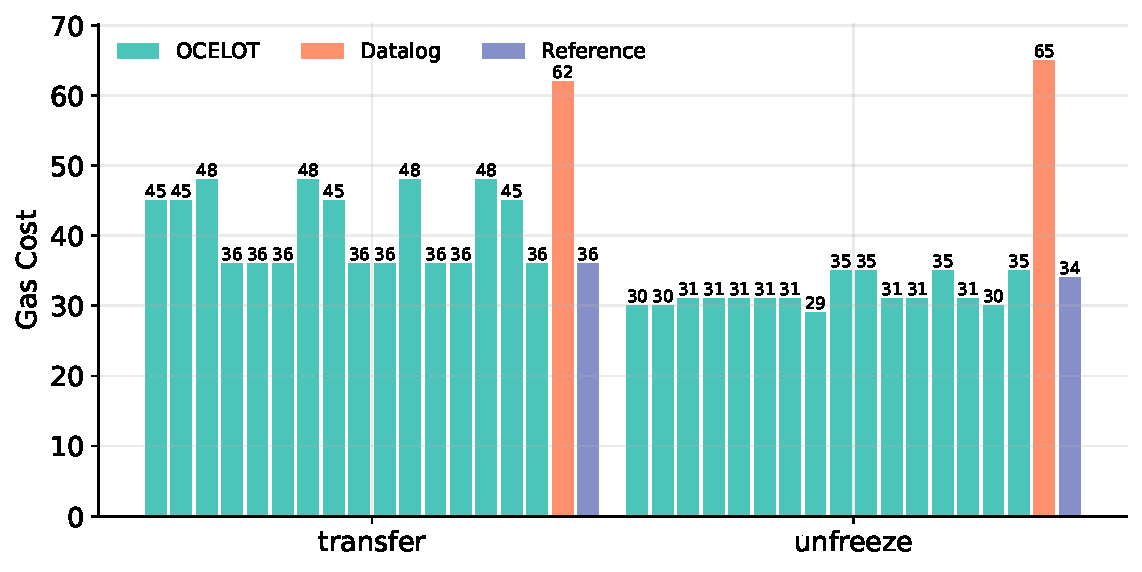
\includegraphics[width=0.5\textwidth]{figures/bnb_functions.pdf}
    \caption{Gas consumption of 2 transactions in BnB contract.}
    \label{fig:bnb-functions}
\end{figure}

\noindent\textbf{Cases where \proto shows improvement over Incremental Datalog and matches Reference.}
Compared with {\sf Incremental Datalog}, \proto lowers gas usage by $>$20\% on 24 of the 35 benchmarks and exceeds 40\% gas saving (up to 70.6\%) on half of the contracts. 
The gain mainly arises from \proto’s selective view materialization, which avoids excessive storage operations that novice Datalog programmers typically leave in place.  

In several cases (e.g.,{\sf WBTC}), \proto even surpasses the manually optimized reference contracts, partially because it applies read projection uniformly, an optimization missing from other implementations.
In a few contracts like \textsf{ERC20} and \textsf{BnB}, \proto underperforms {\sf Reference} by a small margin.  
This performance gap does not come from the additional materialization of relations; instead, it arises from low‑level code optimizations that the current compiler has not yet supported. 
For example, {\sf Reference} contracts rely on in‑place updates (e.g., \lstinline{"a += b"}), whereas \proto expands these operations to \lstinline{"a = a + b"}, which requires an extra read. 
Besides, \proto's current automatic Solidity compiler splits each Datalog rule into separate update functions, introducing additional overhead compared to extensive function inlining in {\sf Reference}. 
Note that these features are not the primary focus of this project, as their impact on the contract's gas cost is deemed insignificant. Moreover, they are well-known standard optimization strategies that can be incorporated into future versions of \proto.


\noindent \textbf{Cases where \proto underperforms the Reference.}
Rarely, \proto shows minimal or no improvement over {\sf Incremental Datalog}, while underperforming the {\sf Reference}.
In these contracts (e.g. \textsf{VestingWallet, Ballot}), the Datalog specification declares only a handful of relations, all of which must be materialized, leaving little room for \proto’s selective‑view heuristics compared to {\sf Incremental Datalog}.  
While our optimization techniques will not harm the performance, there are some special contract logics that are specifically handled and optimized in expert hand-optimized {\sf Reference} but are currently not supported by \proto's automatic compiler.
For example, the contract \textsf{VestingWallet}'s behavior depends on several mutually exclusive conditions. While the {\sf Reference} evaluates the required state once and reuses it across branches, Datalog has to write each branch as a separate rule, forcing \proto to re‑read the same relations for every branch and inflating gas consumption. 
We further provide a detailed gas breakdown analysis on {\sf Voting} contract in Sec ~\ref{ssec:gas-breakdown} to explain the main reasons for \proto's gas overhead compared to {\sf Reference}.
However, these shortfalls here reflect some Datalog semantic and compiler implementation limitations, which can be considered as future optimizations rather than shortcomings of our current optimization algorithm.



\subsection{Gas Breakdown Study} 
\label{ssec:gas-breakdown}
% We perform a gas breakdown study on the {\sf BnB} Transfer transaction to illustrate the effectiveness of our storage optimization techniques. Table ~\ref{tab:gas-breakdown-BNBTransfer} provides the gas consumption breakdown values of the three different benchmarks over the {\sf BnB} Transfer transaction. Note that the transaction fee is a flat fee for all transaction calls.

% Results of {\sf Incremental Datalog} support the argument that when naively compiling the declarative smart contract to Solidity without any optimizations, storage operations are the dominant factor in overall gas usage. 
% Besides, \proto significantly reduces storage and overall gas utilization compared with {\sf Incremental Datalog}, 
% matching that of the reference implementation. 
% Computation cost is also reduced by up to 50\% from the {\sf Incremental Datalog}.
% The computation overhead over reference
% is caused by the code-level optimization discussed earlier.
% While the difference in the {\sf memory others} gas consumption between reference and \proto is due to different event logging mechanisms, 
% this has little impact on the result analysis.
% This result demonstrates the effectiveness of \proto.

\begin{table}[t]
\caption{Gas breakdown of the Voting Vote Transaction}
    \centering
    \footnotesize
    \begin{tabular}{ll|lll}
    \hline
\textbf{Instruction type}         &        & \textbf{Datalog} & \textbf{Ref.} & \textbf{\proto} \\
\hline
\multirow{3}{*}{memory}  & read   & 34                  & 8         & 27         \\
                         & write  & 124                 & 52        & 107         \\
                         & others & 1,262                & 1,716      & 1,262         \\
    \hline
\multirow{2}{*}{storage} & read   & 14,633               & 10,733      & 13,900         \\
                         & write  & 53,480               & 36,933      & 46,780         \\
    \hline
compute                  &        & 3,273               & 1,525      & 3,100         \\
    \hline
transaction fee          &        & 21,570.8
    & 21,570.8     & 21,570.8         \\
    \hline
all                      &        & 94,005               & 71,527    & 86,375         \\
    \hline
\end{tabular}
    \label{tab:gas-breakdown-Vote}
\vspace{-1.5em}
\end{table}

We perform two gas breakdown studies to illustrate the effectiveness and boundaries of our storage optimization techniques. 

Tables ~\ref{tab:gas-breakdown-BNBTransfer} and ~\ref{tab:gas-breakdown-Vote} provide the gas consumption breakdown values of the three different benchmarks over the {\sf BnB} Transfer transaction and the {\sf Voting} Vote transaction. Note that the transaction fee is a flat fee for all transaction calls. Our results support that the gas consumption of storage operations is the dominant factor in overall gas usage. While the main {\sf memory} gas difference in {\sf memory others} comes from different event logging mechanisms, this has little impact on the overall result analysis.

% Results of {\sf Incremental Datalog} support the argument that when naively compiling the declarative smart contract to Solidity without any optimizations, storage operations are the dominant factor in overall gas usage. 
In table ~\ref{tab:gas-breakdown-BNBTransfer}, we show that, for most token-type contracts, \proto significantly reduces storage and overall gas utilization compared with {\sf Incremental Datalog}, matching that of the reference implementation. In this case, {\sf BnB} works as the representative of token contracts that have similar logics, and Transfer is their dominant transaction type. Computation cost of \proto is also reduced by up to 50\% from the {\sf Incremental Datalog}, while the overhead over {\sf Reference} is caused by the code-level optimization discussed earlier.

However, in ~\ref{tab:gas-breakdown-Vote}, we observe that \proto underperforms the reference in both storage and overall gas consumption, though being still more efficient than {\sf Incremental Datalog}. Specifically, we find that the average number of storage read and write over all the traces generated for the Vote transaction in {\sf Incremental Datalog}, {\sf Reference}, and \proto are (13,5), (7.3, 2.7) and (12.3, 4.3) respectively.
We found that the extra storage reads come from redundant reads of the same parameters in different functions, since the automatic compiler translates each rule into a separate function. For example, different functions all require the balance value v of a given user address p, where p can be passed as a parameter during function calls, but each function has to read v separately from p's slot. This issue not only exists in IF-ELSE, but also exists in a more general case when the rule logic becomes more complex.
% Moreover, while people can validate the condition by semantic meanings in some case (for example, if (!isVoter) ), the compiler generated version has to use an extra valid flag to judge if this tuple exists or not. And the extra valid flag will sometimes occupy a new slot, causing more SSLOAD and SSTORE.
Moreover, the compiler-generated code appends an extra valid bit to each record to judge if this record exists or not, while in {\sf Reference}, people can read the context and manually validate the existence of a record by its semantic meaning. 
Take the relation {\sf \lstinline{hasWinner}} as an example:
\[
\texttt{hasWinner(true)} \;:\!- \;
    \texttt{wins(\_,b)}, \texttt{b == true}
\]
Given the default value of {\sf \lstinline{hasWinner}} to be false, the compiler can not distinguish if {\sf \lstinline{hasWinner}} is never updated and is false, or if it is updated to true but again changed to false. Thus, the compiler can not use {\sf \lstinline{hasWinner(false)}} to decide if there have never been any winners. However, the expert can analyze the context and claim that {\sf \lstinline{hasWinner(false)}} equals no winners ever. 
Similarly, given the value of {\sf \lstinline{Votes}} in address p to be 0, the compiler can not tell if it is set to zero or the current record of {\sf \lstinline{Votes(p)}} doesn't exist and thus returns 0 by default. In this case, the compiler has to use {\sf \lstinline{Votes(p)._valid}} to decide.
However, the extra valid bit will sometimes occupy a new storage slot, e.g, when the value of {\sf \lstinline{Votes(p)}} is of unit32 type and fills a 32-bit storage slot entirely on its own, causing extra SSLOAD and SSTORE operations when updated.
Table ~\ref{tab:gas-model} illustrates that each SSLOAD incurs 100-2100 gas, and an extra SSTORE even leads to 22100 extra gas, significantly increasing the overhead. 

These breakdown analyses help to explain why \proto works best for most token type contracts using our view elimination and selective materialization approaches, and show future orthogonal optimization space for advanced contracts with complex conditions.

% This result demonstrates the effectiveness of \proto.

\subsection{Case Study: View Selection}

We present an interesting case study involving the {\sf BnB} contract. After analyzing all versions of the implementation generated by \proto, each corresponding to different minimal materialization plans, we identified a complex performance pattern. Notably, certain versions excel in specific transactions (such as {\sf \lstinline{unFreeze}}), surpassing the reference version, while in other transactions (like {\sf \lstinline{transfer}}), they may perform less effectively. To illustrate this more clearly, Figure~\ref{fig:bnb-functions} shows the results of the 16 \proto versions alongside two other baselines for the {\sf \lstinline{unFreeze}} and {\sf \lstinline{transfer}} transactions.

This behavior can be attributed to the presence of a relation that is updated during the execution of {\sf \lstinline{unFreeze}} and utilized during the execution of {\sf \lstinline{transfer}}. When this relation is not materialized, the maintenance cost for {\sf \lstinline{unFreeze}} can decrease; however, this reduction comes at the cost of a higher query expense for {\sf \lstinline{transfer}}, since the relation must be computed on demand.

\begin{figure}[t]
    \centering
    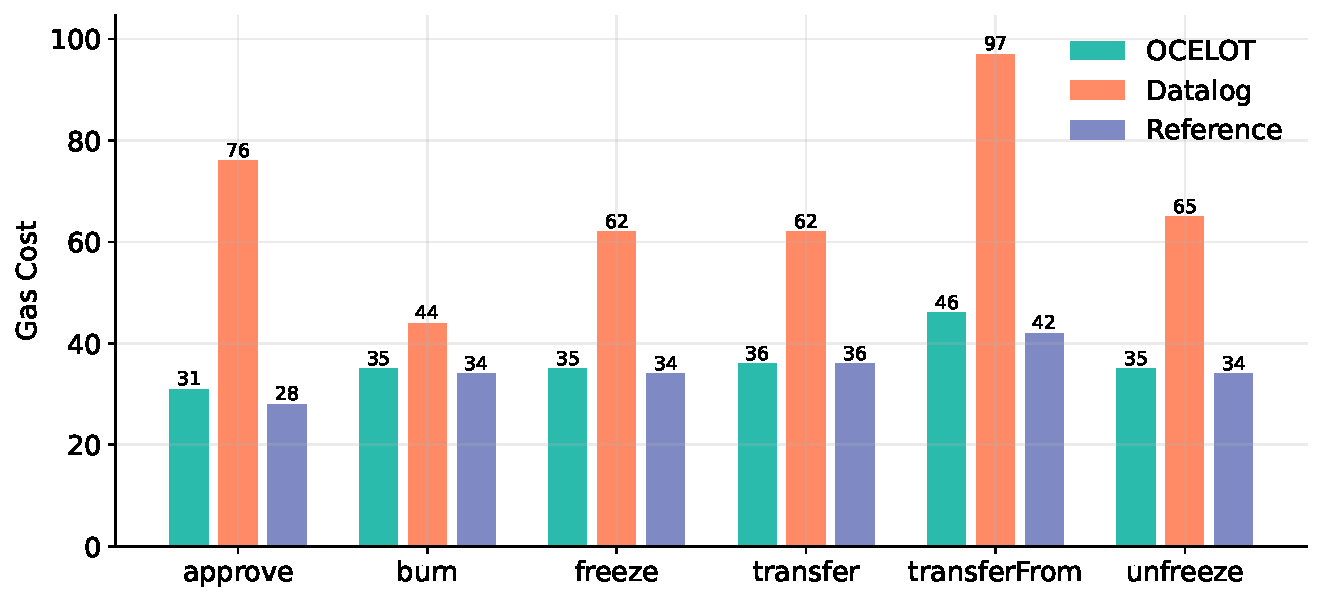
\includegraphics[width=0.5\textwidth]{figures/bnb_best_min.pdf}
    \caption{Gas consumption of the best \proto plan in BnB contract.}
    \label{fig:bnb-best-plan}
\vspace{-1.5em}
\end{figure}

Note that in the long run, \proto prioritizes the version with the overall best gas performance, considering all transactions collectively given their frequencies. As depicted in Figure~\ref{fig:bnb-best-plan}, since {\sf \lstinline{transfer}} is the most frequent transaction in {\sf BnB}, the selected overall optimal \proto version ensures gas efficiency for {\sf \lstinline{transfer}} and may incur slightly more gas consumption for the {\sf \lstinline{unFreeze}} function compared to the {\sf reference} and other \proto plans.